\section{Zielsetzung}

In diesem Versuch soll durch Beobachtung des Phasenübergangs die 
Verdampfungswärme von Wasser bestimmt werden. Dafür wird die Dampfdruckkurve zu Hilfe genommen. Außerdem soll dabei die Temperaturabhängigkeit nicht vernachlässigt werden.

\section{Theoretische Grundlagen}

%\subsection{Phasendiagramm}

Die \glqq Phase\grqq{} eines Stoffes beschreibt in diesem Fall den Aggregatzustand. Wir unterscheiden dabei zwischen fest, flüssig und gasförmig.
Zur Veranschaulichung wird hier ein Phasendiagramm von Wasser genutzt in dem die Temperatur gegen den Druck aufgetragen ist und die 3 \glqq Phasen\grqq{}
durch 3 Kurven voneinander abgegrenzt sind.\\
\begin{figure}[H]
    \centering
    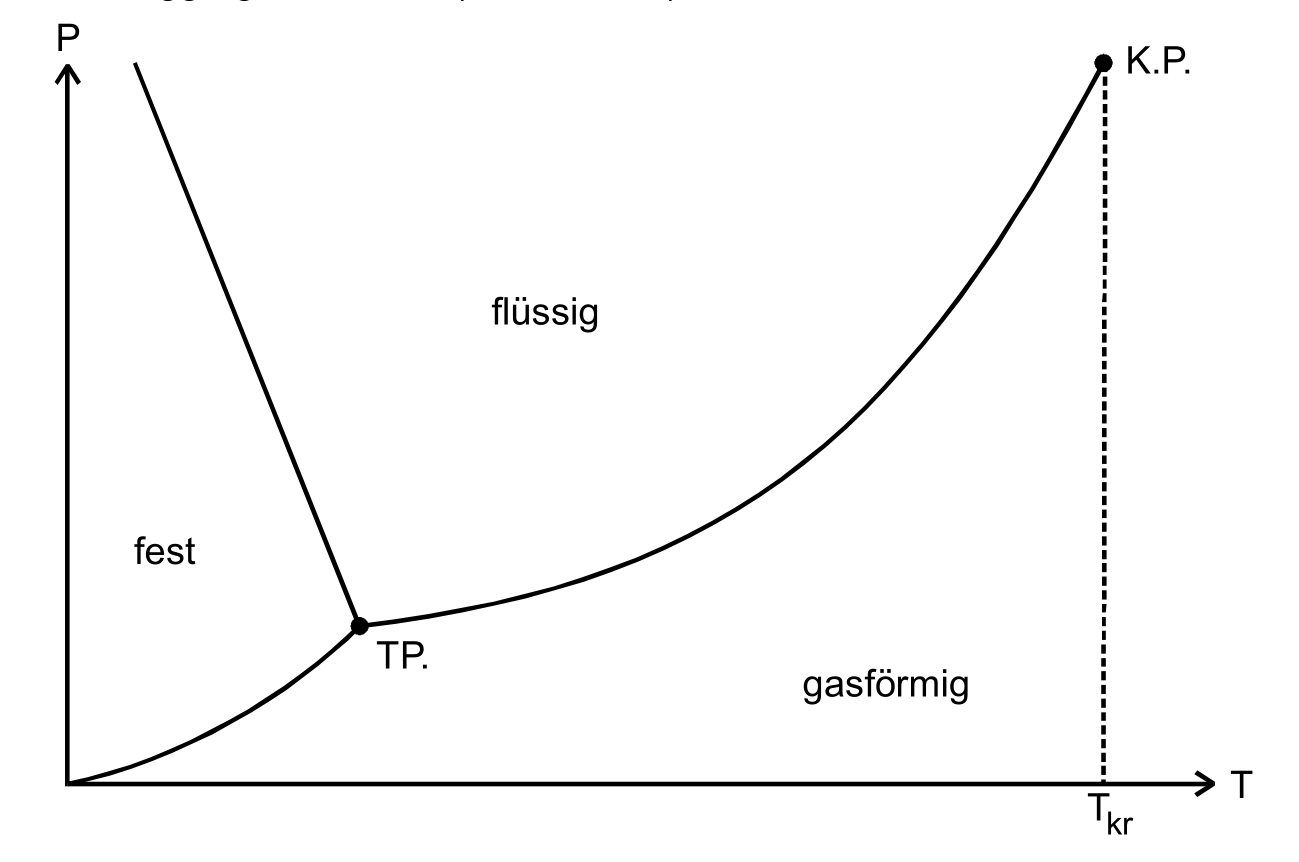
\includegraphics[width=0.55\textwidth]{images/Diagramm.PNG}
    \caption{Zustandsdiagramm des Wassers (qualitativ) \protect \cite{V203}.}
    \label{img:Zustand}
\end{figure}
Die beiden wichtigen Punkte in dem Diagramm sind der Tripelpunkt (TP.), indem die 
3 Aggregatzustände koexistieren und der kritische Punkt (K.P.) in dem der flüssige und gasförmige Zustand in einem 
thermodynamischem Gleichgewicht stehen.\\
In diesem Experiment untersuchen wir jedoch nur den Übergang: flüssig $\Leftrightarrow$ gasförmig. 
Dieser Übergang wird von der Gasdruckkurve beschrieben bzw. von der Siedepunktskurve zwischen dem Triplepunkt und dem kritischem Punkt.
Diese Kurve wird charakterisiert durch die temperaturabhängige Verdampfungswärme $L$. \\
Innerhalb jedes Stoffes werden die Geschwindigkeiten der einzelnen Teilchen
durch die Maxwellsche Geschwindigkeitsverteilung vorgegeben. Sobald die Geschwindigkeit eines Teilchen einen gewissen Grenzwert 
überschreitet, kann es aus der flüssig in die gasförmige Phase übergehen. Bei diesem Übergang müssen molekulare Bindungskräfte überwunden
werden. Dies ist die Verdampfungswärme $L$. Diese Energie wird beim Umkehrprozess, der Kondensation, wieder frei.\\
Zwischen Kondensation und Verdampfung entsteht nach einiger Zeit ein Gleichgewicht mit einem konstantem Sättigungsdruck.
$L$ ist eine temperaturabhängige Größe. Allerdings gibt es einen Temperaturbereich in dem die Verdampfungswärme näherungsweise konstant ist.
Diesen Bereich nutzen wir in diesem Experiment um $L$ zu bestimmen.
\\$\Rightarrow$ Somit beschreibt die molare Verdampfungswärme $L$ eine stoffspezifische Größe , die angibt, wie viel Energie nötig ist,
um ein Mol einer Flüssigkeit isotherm und isobar zu verdampfen.\\
Der Sättigungsdruck lässt sich nicht durch die allgemeine Gasgleichung:
\begin{equation}
    pV=RV\text{,mit }R=\text{allgemeine Gaskonstante }= \SI{8.314}{\joule\per\mole\kelvin}\\
    \label{eqn:Gasgl}
\end{equation}
\\
beschreiben, da der Sättigungsdruck nicht von dem Volumen des Gases, jediglich von der Temperaturen der Flüssigkeit 
und des Gases abhängen.
\\
Um nun auf eine Dampdruckkurve zu kommen, schauen wir uns reversiblen Kreisprozess an. Hier findet in einem fortlaufendem 
Kreislauf eine isotherme und isobare Vedampfung gefolgt von einer isothermen und isobaren Kondensation\\

\begin{figure}[H]
    \centering
    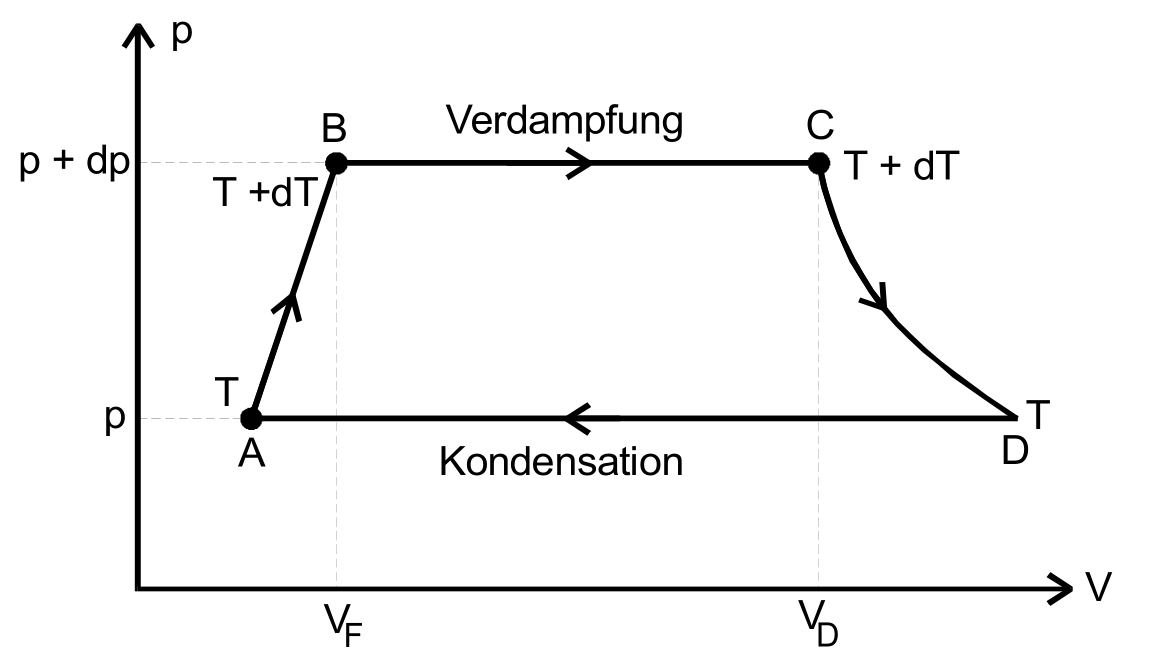
\includegraphics[width=0.55\textwidth]{images/Kreislauf.PNG}
    \caption{Darstellung eines Kreisprozesses im pV-Diagramm \protect \cite{V203}.}
    \label{img:Kreislauf}
\end{figure}

Ausgangspunkt A, die Wärmemenge $\text{dQ}_\text{AB} $ wird hinzugefügt, so dass, der Druck und die Temperatur um dp und dT ansteigen.
Diese Wärmemenge berechnet sich mittels der spezifischen Wearmekapaziteat der Fluessigkeit.
\begin{equation}
    \text{dQ}_\text{AB}= \text{C}_F \cdot dT \nonumber\\
\end{equation}
$\rightarrow$ Zustand B\\
Die Flüssigkeit vedampft isobar und isotherm unter Aufnahme der Verdampfungswärme d$L$\\
\begin{equation}
L\text{(T + dT)} = L\text{(T) + d}L\nonumber\\
\end{equation}
Die in diesem Prozess verichtete Arbeit berechnet sich durch :\\
\begin{equation}
   - \text{A}_\text{BC} = \text{(p + dp)(V}_\text{D} - \text{V}_\text{F}\text{)} 
\end{equation}
$\rightarrow$ Zustand C\\
Durch Wärmeentzug wird der Dampf wieder auf die Temperatur T abgekühlt \\
Bei diesem Schritt wird wieder eine gewisse Wearmemenge $\text{dQ}_\text{CD}$ frei:
\begin{equation}
 -\text{dQ}_\text{CD} = \text{C}_\text{D}\cdot \text{dT} \text{C}_\text{D} = \text{Molarwärme des Dampfes}   
\end{equation}
$\rightarrow$ Zustand D\\
Im letzten Schritt Kondensiert man den Dampf unter Zufuhr der Mechanischen Arbeit $\text{A}_\text{Da}$.
Hierbei wird die Verdampfungswärme L(T) frei\\ 
\begin{equation}
    -\text{A}_\text{Da}= \text{p}\cdot\text{(V}_\text{D} - \text{V}_\text{F}\text{)}
\end{equation}
$\rightarrow$ Zustand A\\
            %weiter Herleitung der Formel

Nach dem ersten Hauptsatz der Thermodynamik dürfen wir nun die Summer der insgesamt hinzugefügt Wärme mit der insgesamt 
verrichteten Arbeit gleichstellen. Dies ergibt dann:        
\begin{equation}
    (C_\text{F}-C_\text{D})dT + dL = (V_\text{D}-V_\text{F})dP\\
    \label{eqn:wearme=Arbeit}
\end{equation}
Nach dem zweiten Hauptsatz ser Thermodynamik ist nun die Summer der reduzierten Wärmemenge gleich 0.

\begin{equation}
    \sum_{i}\frac{Q_\text{i}}{T_\text{i}}=0\nonumber\\
    \label{eqn:sum1}
\end{equation}

Weiterhin dürfen wir die Differentialausdrücke 2. Ordnung vernachlässigen, und erhalten daraus:

\begin{equation}
    \text{(C}_\text{F} - \text{C}_\text{D}\text{)dT + dL }-\frac{\text{LdT}}{T}= 0
    \label{eqn:Wearme=0}
\end{equation}

Das Gleichstellen der Formel \eqref{eqn:wearme=Arbeit} mit der Formel \eqref{eqn:Wearme=0} ergibt dann:

\begin{equation}
    (V_\text{D}-V_\text{F})dp =\frac{L}{T}dT\\
    \label{eqn:Clausius}
\end{equation}
Die erhaltene Formel \eqref{eqn:Clausius} wird in der Literataur als Clausius-Clapeyronische Gleichung bezeichnet. Mit ihrer Hilfe 
lässt sich die Dampfdruckkurve eines Stoffes berechnen. Da insgesamt jedoch die Integration sehr schwierg sein kann,zum Lösen müssen 
zunächst einige Näherungen gemacht werden. Dies lässt sich machen, wenn man sich nur besondere Temperaturbereiche anschaut.
\\
        %Loesung der Clausius Gleichung
\\
\\
Für den Temperaturbereich weit unter der kritischen Temperatur $\text{T}_\text{kr}$ (siehe Abbildung \ref{img:Zustand}) dürfen wir einige Näherungen machen.
\begin{enumerate}
    \item $\text{V}_\text{F}$ ist im Verhältnis zu $\text{V}_\text{D}$ vernachlässigbar.
    \item $\text{V}_\text{D}$ lässt sich durch die ideale Gasgleichung beschreiben \eqref{eqn:Gasgl}\\
            \begin{equation}
                \Rightarrow \text{V}_\text{D} \text{(p, T)} = \text{R}\frac{\text{T}}{\text{R}}
            \end{equation}
    \item Die Verdampfungswärme $L$ ist Druck- und temperaturunabhängig.
\end{enumerate}
Unter diesen Näherungen können wir die Clausius-Clapeyronsche Gleichung \eqref{eqn:Clausius} deutlich Vereinfachen:
\begin{equation}
    \frac{\text{R}}{\text{p}}\text{dp} = \frac{\text{L}}{\text{T}^2}\text{dT}
\end{equation}
\begin{align}
p &= \text{exp}(C)\cdot \text{exp}\left(-\frac{L}{R \cdot T}\right)\\
\text{ln}(p)&= -\frac{L}{RT} + C
\end{align}
mit $C$ = ln($\text{p}_0$)
